For the problems we have considered thus far, the eigenvalues have always
satisfied nice formulas that are fairly easy to compute.  This problem 
illustrates that this is not always the case.  
%(But if you can compute
%the eigenvalues and eigenfunctions to good accuracy, the spectral method 
%will work just like normal.)

Consider the equation
\[ -u''(x) = f(x), \quad x\in[0,1] \]
with a homogeneous \emph{Robin condition} on the left,
\[ u(0) - u'(0) = 0\]
and a homogeneous Dirichlet boundary condition on the right,
\[ u(1) = 0.\]

Define the linear operator $L: V\to C[0,1]$ via $Lu = -u''$ with
\[ V = \{u\in C^2[0,1]:  u(0)-u'(0)=u(1)=0\}.\]

\begin{enumerate}
\item Prove that $L$ is symmetric.

\vspace*{1em}
\item Is zero an eigenvalue of $L$?  That is, does there exist a 
      nontrivial solution to $-u''(x) = 0$ with these boundary conditions?

\vspace*{1em}
\item Compute the eigenfunctions of $L$ associated with nonzero eigenvalues, 
      and show that these eigenvalues 
      $\lambda$ must satisfy the equation
      \[ \sqrt{\lambda} = - \tan(\sqrt{\lambda}).\]

\vspace*{1em}
\item In MATLAB, create a plot of $g(x) = -\tan(x)$ for $x\in [0, 5\pi]$ 
      and superimpose (\verb|hold on|) a plot of $h(x)=x$.
      By hand, mark the points where these two functions intersect on your plot.

\vspace*{1em}
\item Use your plot in~(d) to argue that $L$ has infinitely many eigenvalues, \\
      with $(n-{1\over 2})^2@\pi^2 < \lambda_n < (n+{1\over2})^2@\pi^2$.
      What value does $\lambda_n$ tend to as $n$ becomes large?

\vspace*{1em}
\item Estimate the first four eigenvalues to at least six digits of accuracy.\\
      You will need to find the points of intersection you marked in part~(d).\\
      Please \emph{don't} just try to `eyeball' these by zooming in on your plot!\\
      Instead, either use MATLAB's \verb|fzero| function, or write your
      own implementation of a root-finding algorithm (Newton's method, 
      bisection, etc.).

\item {[optional: 5 bonus points]}\\
      Recall the finite difference matrices you worked with in Problem Set~3.
      Figure out how to construct a similar discretization of 
      $L \psi = \lambda \psi$ for the linear operator in this problem,
      paying particular attention to the boundary condition at $x=1$.
      You should arrive at a matrix equation
      of the form $\BD \Bv = \lambda \Bv$.  
      Compute the eigenvalues of $\BD$
      using MATLAB's \verb|eig| command.  How do these approximations
      compare to the values you computed in part~(f), as you take finer
      and finer discretizations ($N\to\infty$)\,?
      
      Hint:  The first row of your matrix equation $\BD\Bv = \lambda \Bv$ should
      encode the equation
      \[ {-u_0 + 2 u_1 - u_2 \over h^2} = \lambda u_1.\]
      Obtain a formula for $u_0$ in terms of $u_1$ and $u_2$ via 
      the boundary condition $u(0)-u'(0) = 0$ and the approximation
      \[ u'(0) = {-3u_0 + 4u_1 - u_2 \over 2h} + O(h^2),\]
      and use these values to update the $u_1$ and $u_2$ entries in the 
      first row of $\BD$\ldots.
     
\vspace*{1em}
\end{enumerate}
%%%%%%%%%%%%%%%%%%%%%%%%%%%%%%%%%%%%%%%%%%%%%%%%%%%%%%%%%%%%%%%%%%%%%%%%%%%%%%%%

\ifthenelse{\boolean{showsols}}{\begin{solution}
\begin{enumerate}
\item Suppose $u,v \in V$, so that $u(0)-u'(0)=v(0)-v'(0)=u(1)=v(1)=0.$
      Then integrating by parts twice,
\begin{eqnarray*}
 (Lu,v) &=& \int_0^1 -u''(x)v(x) \,dx \\[0.5em]
        &=& \Big[ -u'(x)v(x)\Big]_0^1 + \int_0^1 \int_0^1 - u'(x)v'(x)\,dx, \\[.5em]
        &=& u'(1)v(1)-u'(0)v(0) + \int_0^1 \int_0^1 - u'(x)v'(x)\,dx,\\[.5em]
        &=& u'(1)v(1)-u'(0)v(0) + \Big[ u(x)v'(x)\Big]_0^1 - \int_0^1 - u(x)v''(x)\,dx\\[.5em]
        &=& u'(1)v(1)-u'(0)v(0) + u(0)v'(0)-u(1)v'(1) - (u,Lv)\\[.5em]
        &=& -u'(0)v(0) + u(0)v'(0) - (u,Lv).
\end{eqnarray*}
In the last step, two boundary terms are zero because $u(1)=v(1)=0$.
For the other boundary term, note that $v(0)-v'(0)=0$ implies $v(0)=v'(0)$,
so $-u'(0)v(0) + u(0)v'(0) = u(0)v(0) - u'(0)v(0) = (u(0)-u'(0))v(0) = 0$
since $u(0)-u'(0)=0$.  Hence $(Lu,v) = (u,Lv)$, so $L$ is symmetric.

[\textbf{GRADERS}: Please deduct 3 points if students do not clearly explain why
the boundary term at $x=0$ is zero.]

\item Zero is \emph{not} an eigenvalue of $L$.  To see this, 
      we seek a nonzero solution $\psi\in V$ to $L\psi = 0 \psi$, i.e., $-\psi''(x) = 0$.
      The general solution of $-\psi''(x) = 0$ is $\psi(x) = A x + B$.
      The right boundary condition $\psi(1)=0$ implies that 
       \[ 0 = \psi(1) = A + B,\]
      hence $A = -B$.  The left boundary condition implies
       \[ 0 = \psi(0) - \psi'(0) = B - A,\]
      hnece $A=B$.  The only solution to both boundary conditions is hence
      $A=B=0$, so the trivial solution $\psi(x) = 0$ is the only solution 
      of $L\psi = 0$ in $V$.
      Thus zero is not an eigenvalue of $L$.

\item We now know that all eigenvalues $\lambda$ are nonzero.  For $\lambda\ne 0$,
      the general solution of $L\psi = \lambda \psi$, i.e. $-\psi'' = \lambda \psi$,
      has the form
      \[ \psi(x) = A \sin(\sqrt{\lambda} x) + B \cos(\sqrt{\lambda} x).\]
      The left boundary condition gives
      \[ 0 = \psi(0) - \psi(1) = A \sin(\sqrt{\lambda} 0) + B \cos(\sqrt{\lambda} 0)
                                - A \sqrt{\lambda} \cos(\sqrt{\lambda} 0)
                                + B \sqrt{\lambda} \sin(\sqrt{\lambda} 0)
                               = B - A \sqrt{\lambda},\]
      hence $B = A \sqrt{\lambda}$.
      The right boundary condition gives
      \[ 0 = \psi(1) = A \sin(\sqrt{\lambda}) + B \cos(\sqrt{\lambda}).\]
      Substituting the left boundary condition into this last formula, we find
       \[ 0 = A \sin(\sqrt{\lambda}) + A \sqrt{\lambda} \cos(\sqrt{\lambda}).\]
      Since we need $A\ne 0$ to obtain nontrivial solutions, this equation implies
       \[ \sqrt{\lambda} = - {\sin(\sqrt{\lambda}) \over \cos(\sqrt{\lambda})}
                         = -\tan(\sqrt{\lambda}).\]

\item The plot is shown below.  The code that produced it follows at the end
      of this solution.

\begin{center}
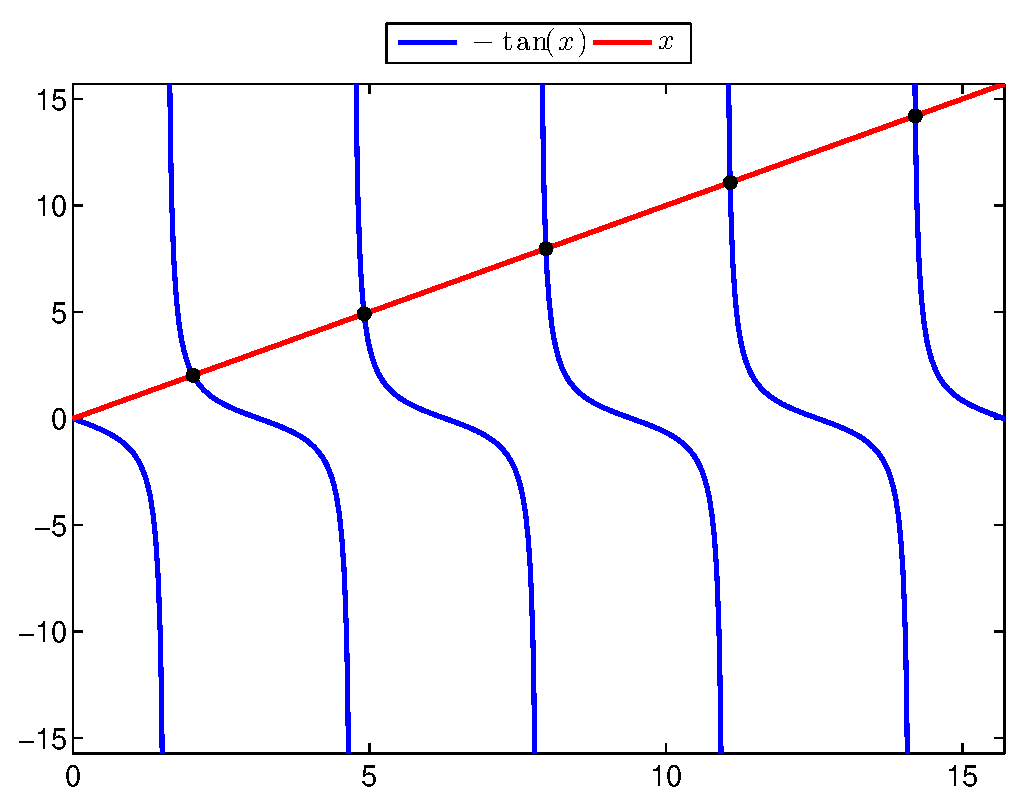
\includegraphics[scale=0.7]{eigroot}
\end{center}
      
\item On every interval $((n-{1\over2})\pi, (n+{1\over2})\pi)$, the function $-\tan(x)$
      takes on every value on $(-\infty,\infty)$ exactly once, so there will be precisely
      one intersection between $-\tan(x)$ and $x$ on each of these intervals.
      Hence, exactly one eigenvalue falls in every interval 
       $((n-{1\over2})^2\pi^2, (n+{1\over2})^2\pi^2)$.
      As $x$ gets larger and larger, this intersection occurs closer and closer to the
      left end of the interval, so as $n\to\infty$, we expect 
      \[ \lambda_n \approx (n-\textstyle{1\over2})^2\pi^2.\]

\item Since the plot shows 5 points of intersection for $\lambda>0$, we compute 
      the first 5 eigenvalues, even though the problem only asks for the first four.
      The table below also compares the eigenvalue to the $(n-{1\over2})^2\pi^2$
      as discussed in the last subproblem (not required).

\begin{center}\begin{tabular}{rrrr}
  $n$ & \multicolumn{1}{c}{$\sqrt{\lambda_n}$} & \multicolumn{1}{c}{$\lambda_n$} & \multicolumn{1}{c}{$(n-1/2)^2 \pi^2$} \\ \hline
1 &    2.0287578381 &    4.1158583657 &   2.4674011003 \\
2 &    4.9131804394 &   24.1393420304 &  22.2066099025 \\
3 &    7.9786657124 &   63.6591065504 &  61.6850275068 \\
4 &   11.0855384065 &  122.8891617619 & 120.9026539133 \\
5 &   14.2074367252 &  201.8512583003 & 199.8594891221
\end{tabular}\end{center}

MATLAB's {\tt fzero} works for some of these roots, but the rapid rate of
growth of $-\tan(x)$ causes this algorithm to perform poorly for some roots.
Hence we turned to the bisection algorithm, which includes
the root between two points, and successively cuts that interval in half
as it zeros in on the root.  
This algorithm is not as fast as {\tt fzero}, but is more reliable.

[\textbf{GRADERS}: Please deduct 2 points if students got some incorrect
roots using {\tt fzero} and didn't note that these roots are wrong.
If they got some roots correct but noted that there was a problem 
with {\tt fzero} for some of the roots, you can give full credit.
Please deduct one point if students only report $\sqrt{\lambda_n}$ 
and not $\lambda_n$ as requested in the problem.]

\input eigroot_code

\item {[bonus question]}
The eigenvalues of $\BD$ for various values of $N$ are plotted below.
Indeed, we see increasingly accurate approximations to the eigenvalues 
computed via a completely different method in part~(f).

\begin{tabular}{r rrrrr}
\multicolumn{1}{c}{$N$} &
\multicolumn{1}{c}{$\lambda_1$} &
\multicolumn{1}{c}{$\lambda_2$} &
\multicolumn{1}{c}{$\lambda_3$} &
\multicolumn{1}{c}{$\lambda_4$} &
\multicolumn{1}{c}{$\lambda_5$}\\ \hline
   8 &    4.0841721152 &    23.7107767862   &    61.0866729525 &   112.5994697441 &   171.7282531156 \\ 
  16 &    4.1058135169 &    23.9757051976   &    62.7295637315 &   119.5758989350 &   192.8815393298 \\ 
  32 &    4.1130303588 &    24.0887676846   &    63.3662538535 &   121.8628790245 &   199.1474454253 \\ 
  64 &    4.1151083041 &    24.1253264546   &    63.5766828167 &   122.5995099114 &   201.0898102312 \\ 
 128 &    4.1156652470 &    24.1356573886   &    63.6372636884 &   122.8121852697 &   201.6487031669 \\ 
 256 &    4.1158093721 &    24.1383977521   &    63.6534869375 &   122.8693278028 &   201.7990311254 \\ 
 512 &    4.1158460272 &    24.1391030403   &    63.6576815597 &   122.8841286367 &   201.8380002820 
\end{tabular}

\end{enumerate} 
\end{solution}}{}

